\subsection{ROS - Universe}

%\begin{frame}
%  \frametitle{ROS - Universe}

%\begin{itemize}
% \item Meta operating system for robotics
% \item Obtain, build, write, and run code across multiple computers, and multiple robots
% \item ROS \& ROS-Pkgs a creation of Willow Garage, Inc.
% \item 3D Gazebo simulation, Stage   
%\end{itemize} 
%\end{frame}

%\begin{frame}
%  \frametitle{ROS - Universe (cont'd)}

%\begin{itemize}
% \item Supported platforms: Linux, MacOS, partial support for Windows (Ubuntu!!!)
% \item Languages: C/C++, python, octave, lisp, ~java
% \item Hardware suggested: many cores, nVidia video card for simulation
%\end{itemize} 
%\end{frame}

\begin{frame}
  \frametitle{ROS - Universe}

\begin{itemize}
 \item Packages are the main unit for organizing software
 \item Manifests (manifest.xml) provide metadata about a package, including dependencies, language-specific information such as compiler flags
 \item Stacks are collections of packages that provide aggregate functionality
 \item Stack manifest (stack.xml) provide data about stack, including its dependencies on other stacks
 \item Message descriptions, define the data structures for messages sent in ROS
 \item Service descriptions, define the request and response data structures for services in ROS
\end{itemize} 
\end{frame}

\begin{frame}
  \frametitle{ROS - Universe (cont'd)}

\begin{itemize}
 \item Nodes are combined together into a graph and communicate with one another
 \item ROS Master provides naming and registration services to the rest of the nodes in the ROS system
 \item Nodes communicate with each other by passing messages. A message is a simply a data structure, comprising typed fields
 \item Topics are named buses over wich nodes exchange messanges based on publish / subscribe policy
 \item Service request / reply is done via a Service, which is defined by a pair of messages 
\end{itemize} 
\end{frame}

\section{PR2 - Short Overview}

\begin{frame}
  \frametitle{PR2 - Evaluation Platform}

\begin{itemize}
 \item PR2 as a main platform for evaluation
 \item Gazebo simulation
 \item ROS as a common framework
 \item Using/modification/improvement of existing stacks
 \item Integration of new algorithms and methods as a ROS-stacks   
\end{itemize}

\vspace{1ex}\hspace{42ex}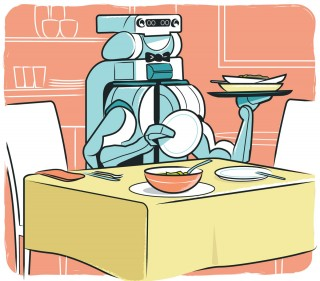
\includegraphics[width=3.5cm]{../images/pr2_dinnertable.jpg} 
\end{frame}

\subsection{PR2 - Hardware Specification}
\begin{frame}
  \frametitle{PR2 - Hardware Specification}
\begin{itemize}
    \item $2\times$ computers with 24 GB RAM and quad-core Nehalem processors
    \item 1.3 kWh Lion Battery Pack
    \item 2 hrs Approximate Runtime
    \item Coordinate system (for all links) positive z-axis up, positive x-axis forward, and positive y-axis robot-left when PR2 in the home pose
    
\end{itemize}

\hspace{12ex}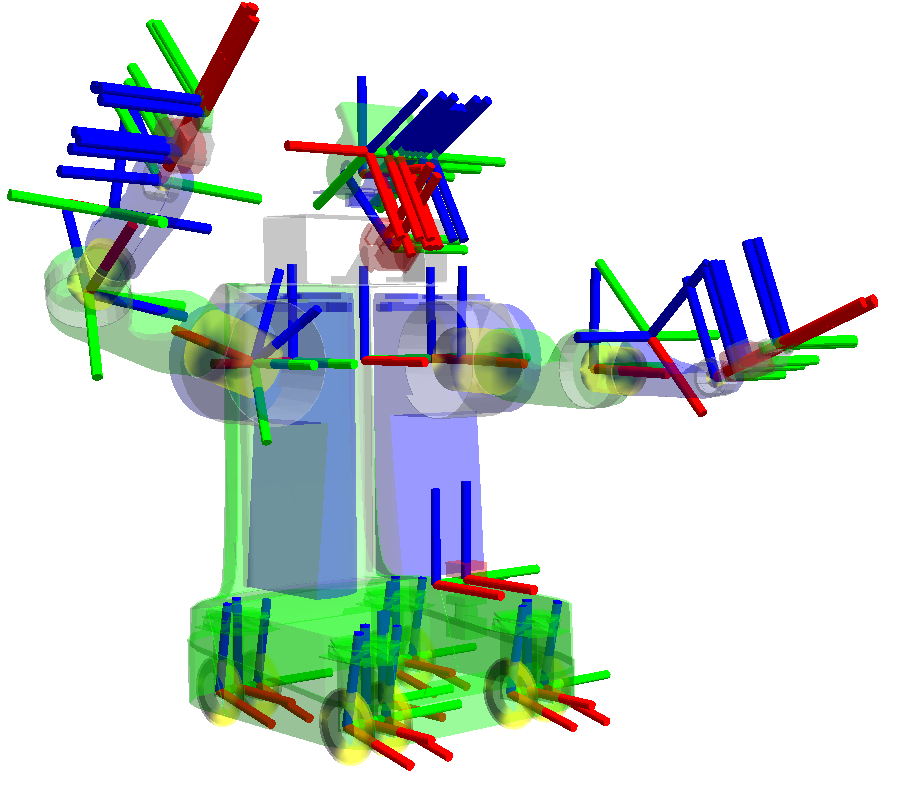
\includegraphics[width=3.5cm]{../images/pr2_frames.png}
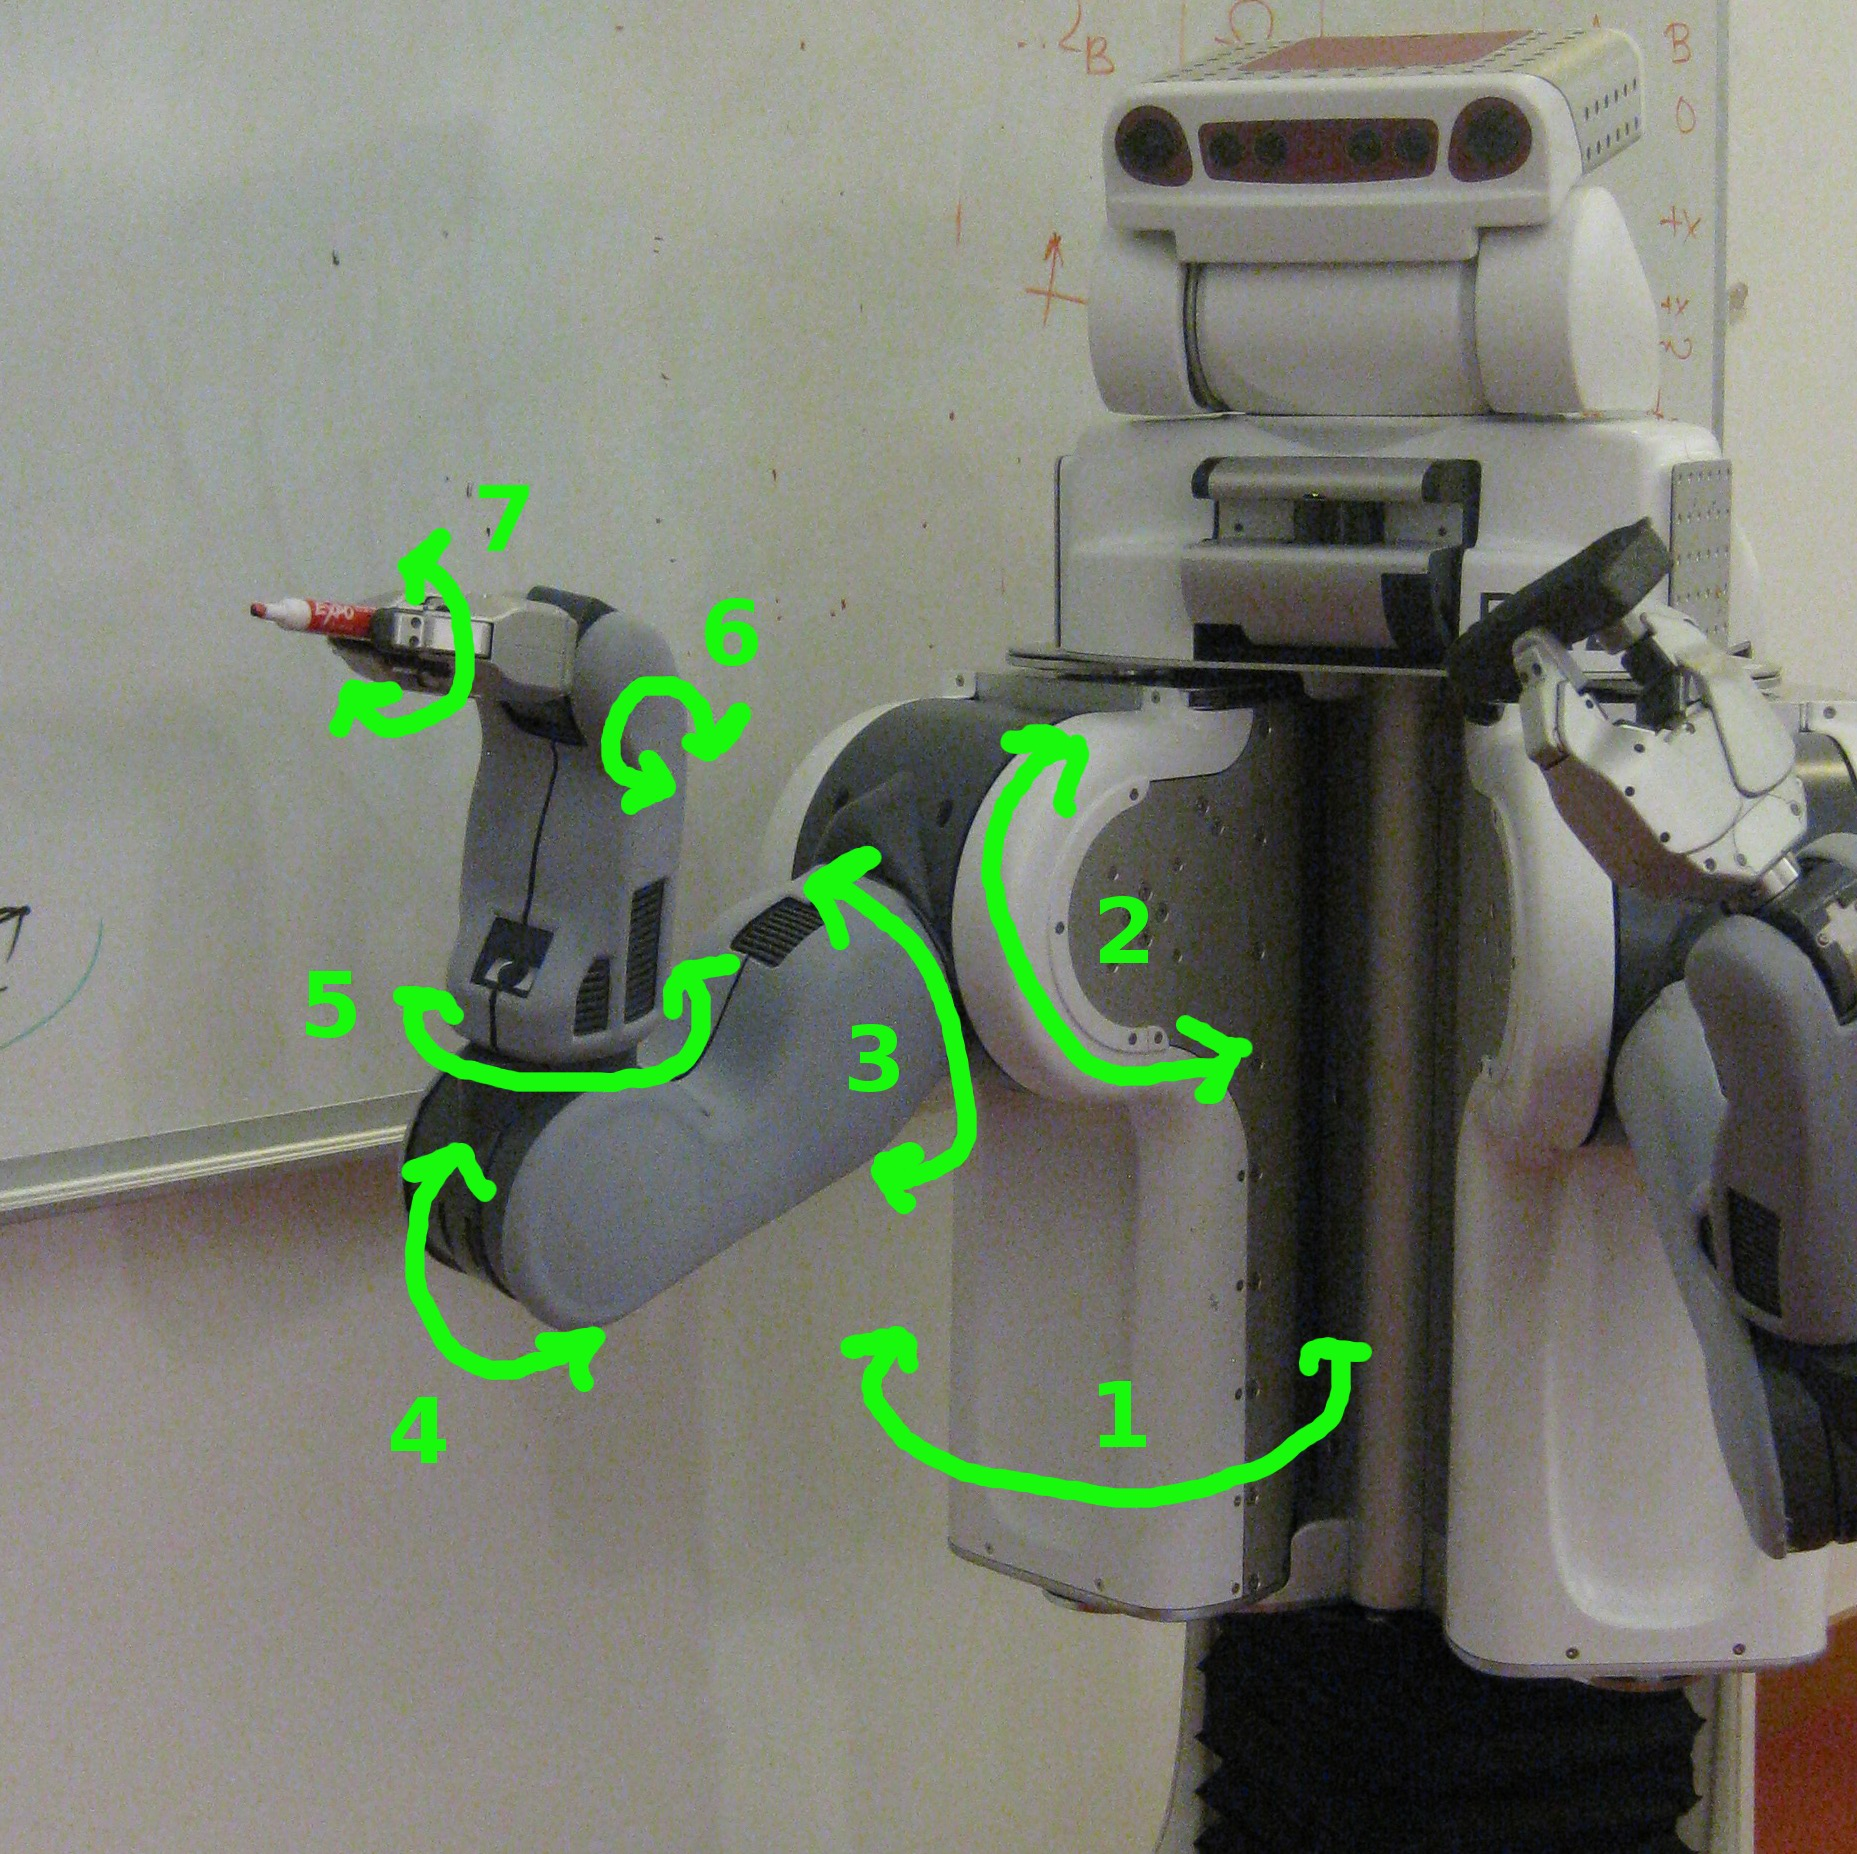
\includegraphics[width=3cm]{../images/pr2arm_dof.jpg}
\end{frame}

\begin{frame}
  \frametitle{PR2 - Hardware Specification}
\small{
\begin{itemize}
    \item Arm DOFs: arm 4 (A), wrist 3 (B), gripper 1 (C)
    \item Link Lengths: upper arm 400\,mm, forearm 321\,mm,\\ wrist to gripper surface 120 - 200\,mm
    \item Range of motion: shoulder pan/tilt $170^0/115^0$,\\ upper arm roll $270^0$, elbow flex $140^0$, forearm \\roll continuous, wrist pitch/roll $130^0$/continuous, \\gripper 90\,mm max
    \item Force output: 4 DOF passive counterbalance, \\arm payload 1.8\,Kg, wrist torque 4\,Nm, \\grip force 80\,N
    
\end{itemize}
}
\vspace{-13ex}\hspace{47ex}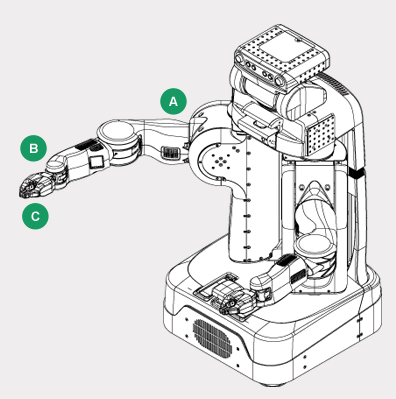
\includegraphics[width=3.4cm]{../images/pr2_arm.png} 
\end{frame}

\subsection{PR2 - Sensors}
\begin{frame}
  \frametitle{PR2 - Intrinsic sensors}
\begin{itemize}
    \item Microstrain 3DM-GX2 IMU (above the shoulders)
    \item Three-Axis Accelerometer (gripper)
    \item Calibration LED (gripper) 
\end{itemize}
\end{frame}

\begin{frame}
  \frametitle{PR2 - Extrinsic sensors - Head}
\begin{itemize}
    \item Microsoft Kinect and/or ASUS Xtion Pro Live (color/depth image/point cloud $[640\times480 @ 30\,fps]$)
    \item Global shutter color gigabit ethernet camera (Prosilica GC2450C, 5\,MP, $[2448\times2050 @ 15\,fps]$)
    \item Wide stereo camera system (Aptina MT9V032C12STC, 100\,Mb color ethernet, $[752\times480@15\,fps]$)
    \item Narrow stereo system (Aptina MT9V032C12STM, 100\,Mb monochrome ethernet, $[752\times480@15\,fps]$)    
    \item LED textured light projector (triggered with narrow-angle stereo camera)
\end{itemize}
\end{frame}

\begin{frame}
  \frametitle{PR2 - Extrinsic sensors - II}
\begin{itemize}
    \item Tilting laser scanner (Hokuyo UTM-30LX, $135^0 (+90^0 to -45^0)$,above the shoulders)
    \item Laser scanner (Hokuyo UTM-30LX, base)
    \item Global shutter gigabit ethernet camera ($2\times$, forearm)
    \item Fingertip pressure sensor arrays (gripper)
    \item Speaker
\end{itemize}
\hspace{-4ex}
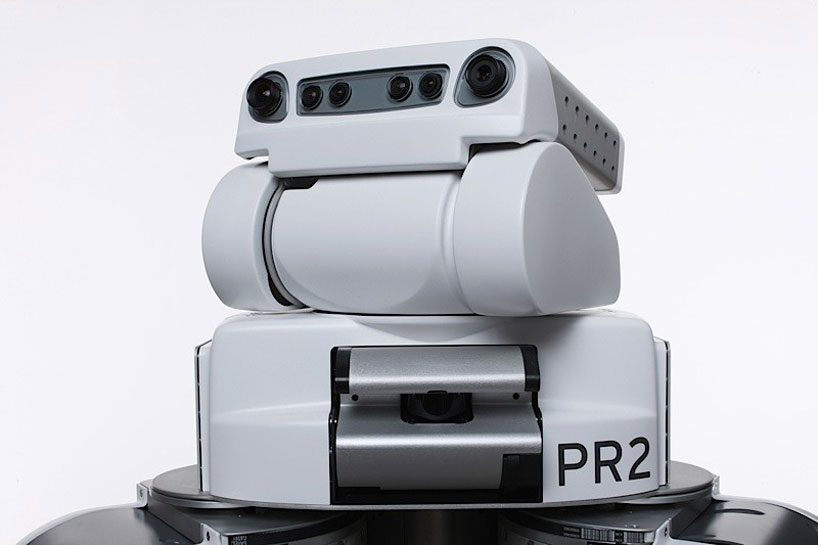
\includegraphics[width=4cm]{../images/head_tiltLRF.jpg} 
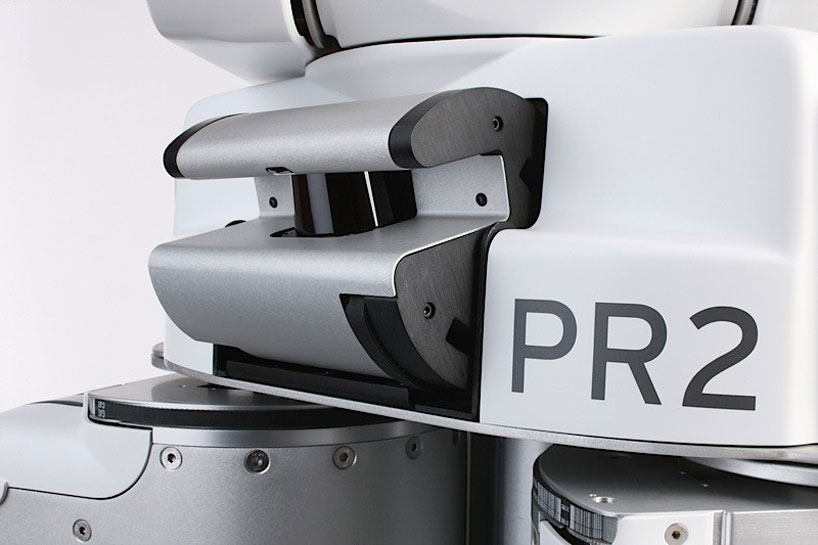
\includegraphics[width=4cm]{../images/tilted_lrf.jpg}
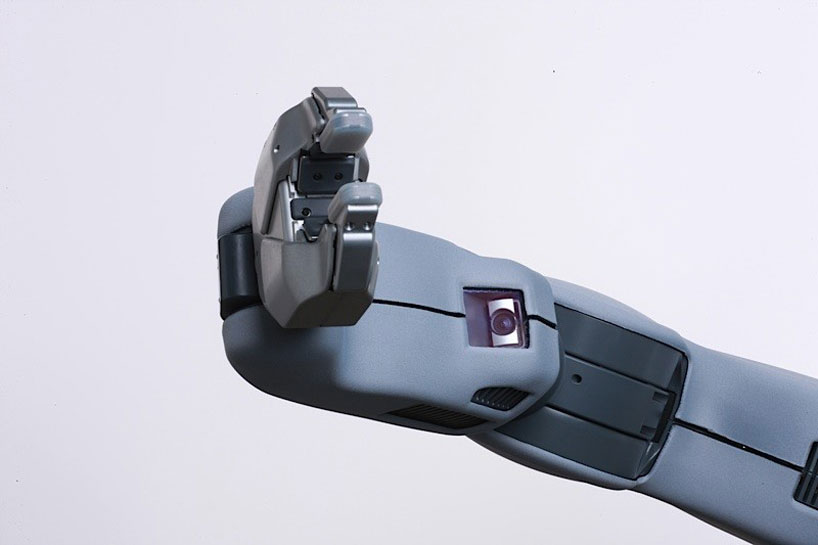
\includegraphics[width=4cm]{../images/pr2_hand_camera.jpg}  
\end{frame}

\begin{frame}
  \frametitle{PR2 - Fingertip pressure sensor arrays (gripper)}
\begin{itemize}
    \item Each PR2 gripper is equipped with 2 pressure-sensitive fingertips
    \item Each pressure comprises 22 pressure sensing elements \\(1 on the back, 6 around the edges, and a $3 \times 5$ array on the front)
\end{itemize}
\vspace{2ex}\hspace{6ex}
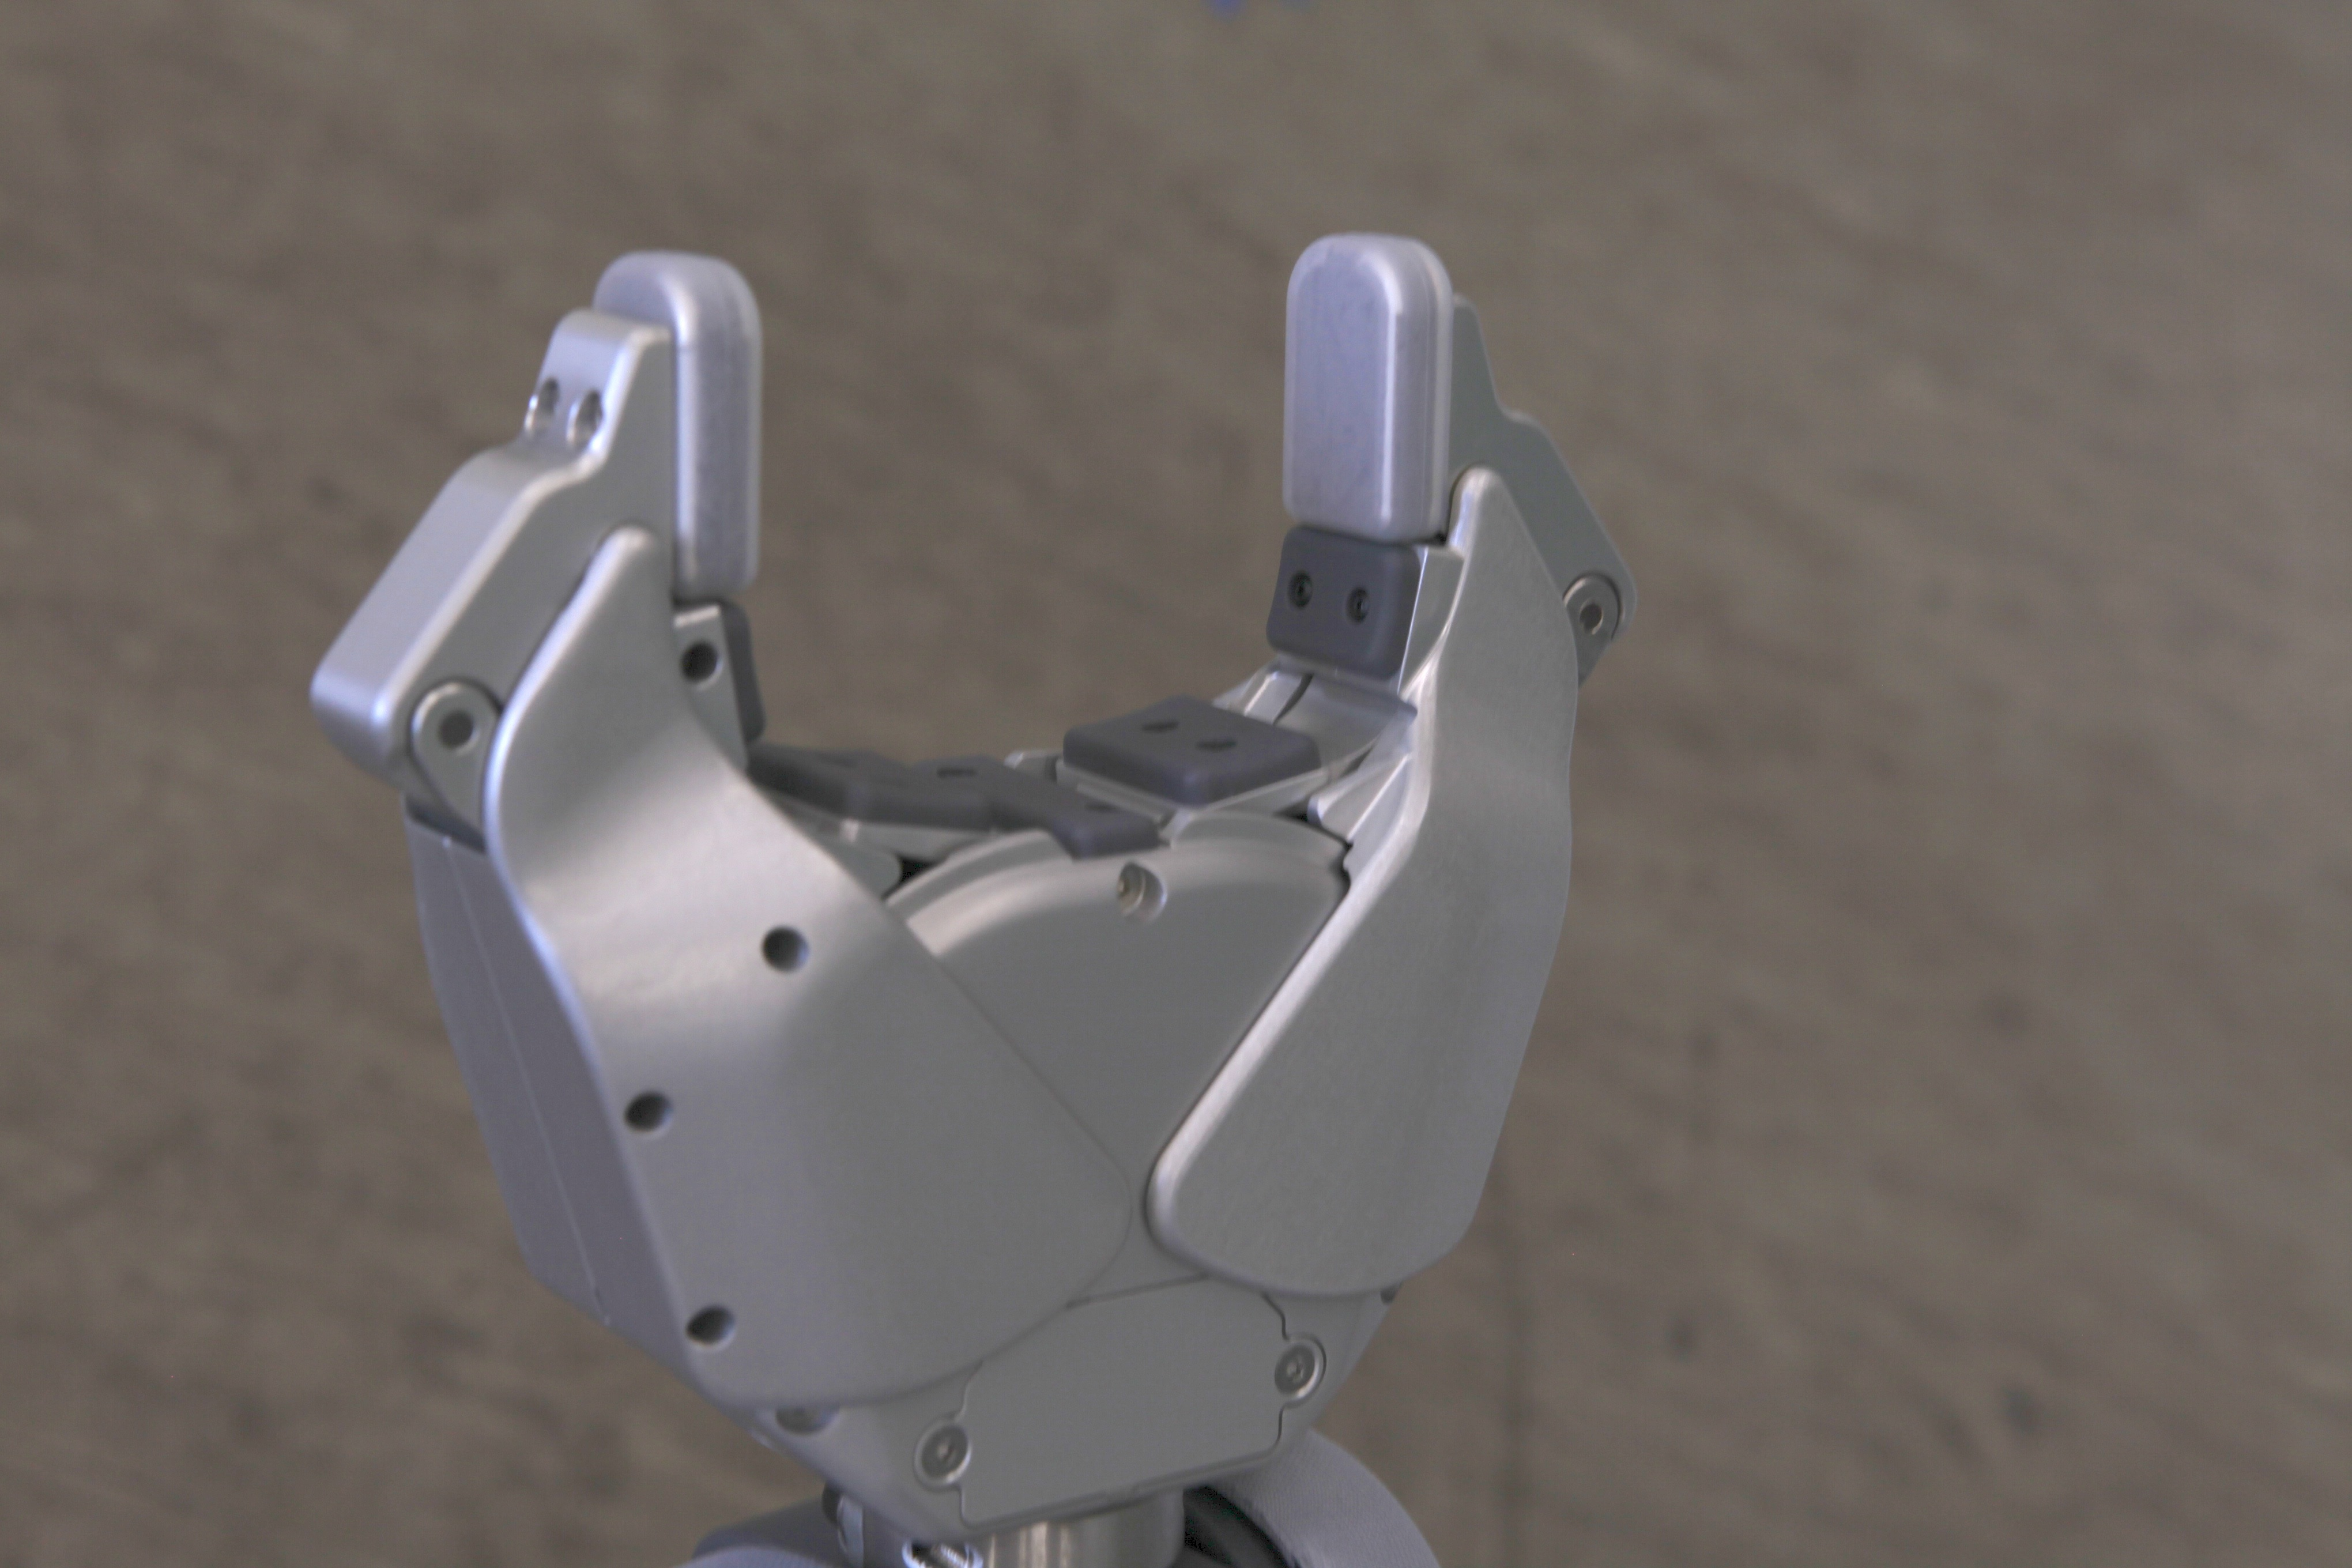
\includegraphics[width=4cm]{../images/IMG_1208.JPG} \hspace{1ex}
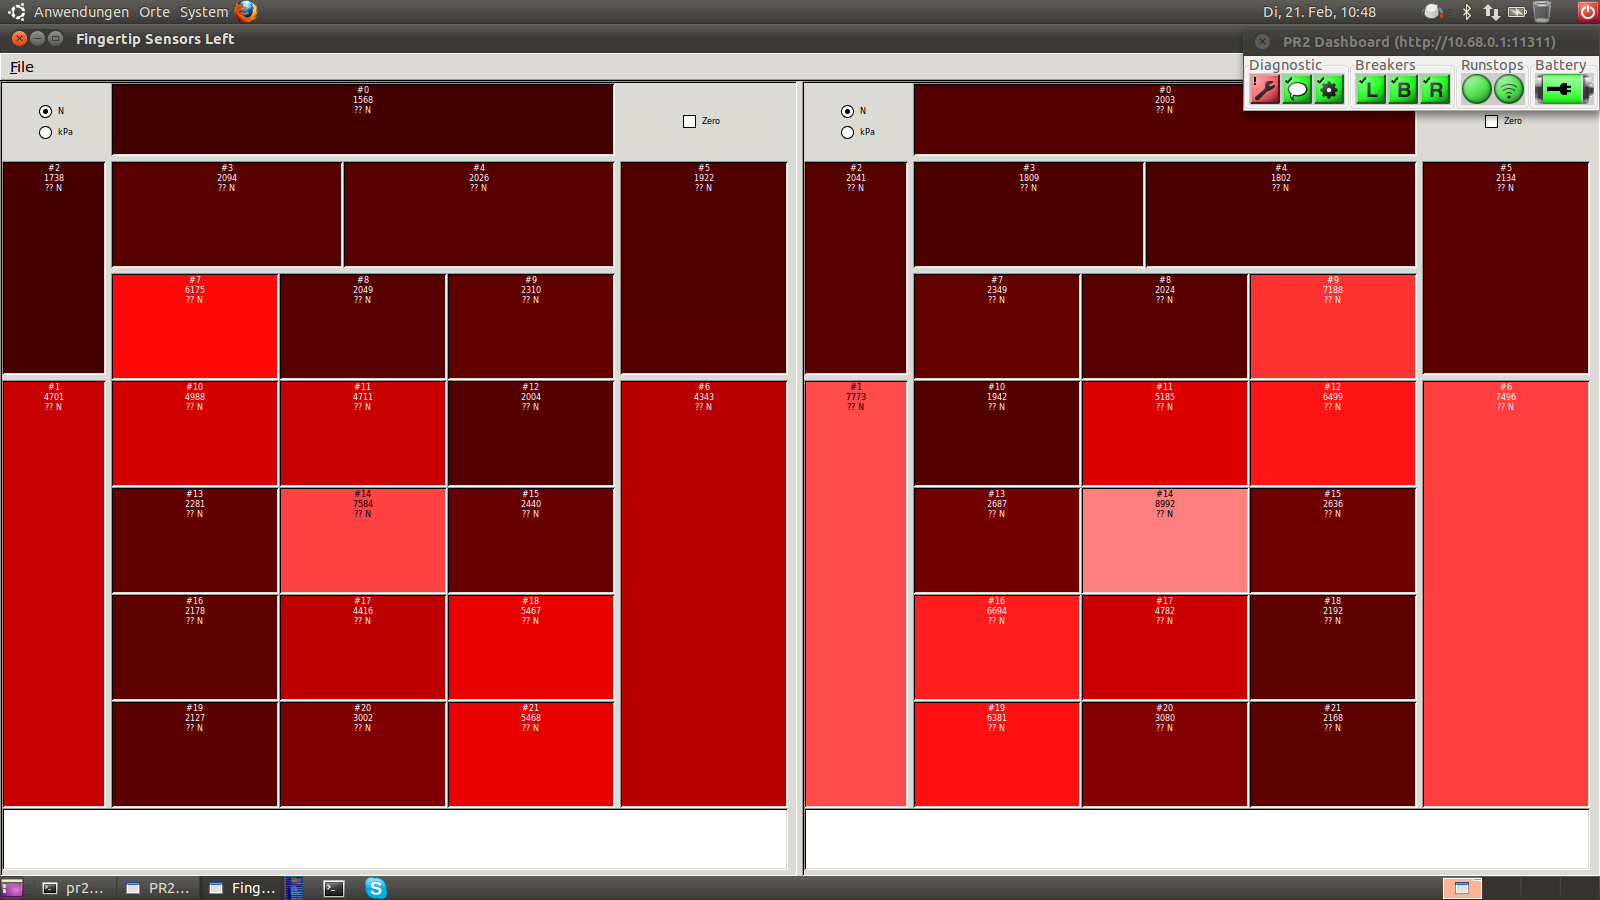
\includegraphics[width=4.75cm]{../images/fingertip_pressure3.png}  
\end{frame}



\section{Extended Sensors}

\subsection{Microsoft Kinect}
\begin{frame} 
 \frametitle{Kinect}
\begin{itemize}
 \item Motion sensing input device by Microsoft for the Xbox 360 video game console
 \item Range camera technology by Israeli developer PrimeSense
 \item 3D scene information from a continuously-projected infrared structured light
\end{itemize}
\hspace{7ex}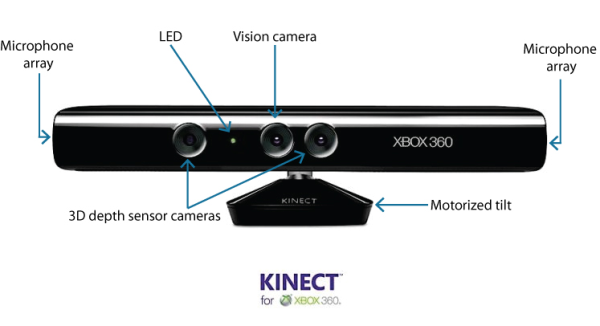
\includegraphics[width=5cm]{../images/Kinect-resized.png} \hspace{1ex}
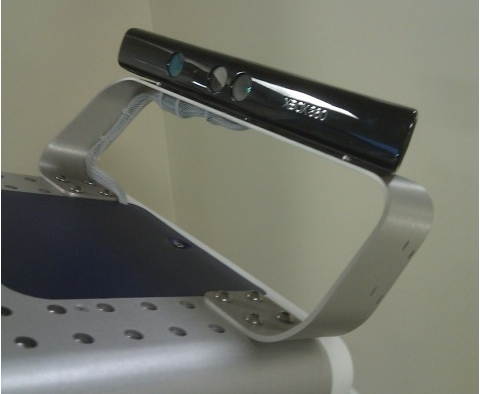
\includegraphics[width=3cm]{../images/PR2_Kinect_spoiler2.jpeg}
\end{frame}

\begin{frame}
 \frametitle{Kinect - technical details}
\begin{itemize}
  \item Resolution of (640 $\times$ 480) @ 30 Hz (color) and (320 $\times$ 240) @ 30 Hz (depth)
  \item Angular field of view of $57^0$ horizontally and $43^0$ vertically
  \item Range of approximately 0.7 - 6\,m (practical 0.7 - 3.5\,m)
  \item Physical tilt range ($-31^0$  to $+31^0$ )
  \item Voice microphone and array supporting single speaker voice recognition (16-bit audio @ 16 kHz)
  \item OpenNI and Freenect drivers
\end{itemize}

\end{frame}

\begin{frame}
 \frametitle{Microsoft Kinect vs. ASUS Xtion Pro Live}
\begin{itemize}
  \item The Xtion Pro Live is significantly smaller
  \item The placement of the lenses are more symmetric \\(this give it a less lopsided appearance and makes it much more usable for humanoids)
  \item The Xtion Pro Live does not require an external power supply
\end{itemize}
\vspace{3ex}\hspace{6ex}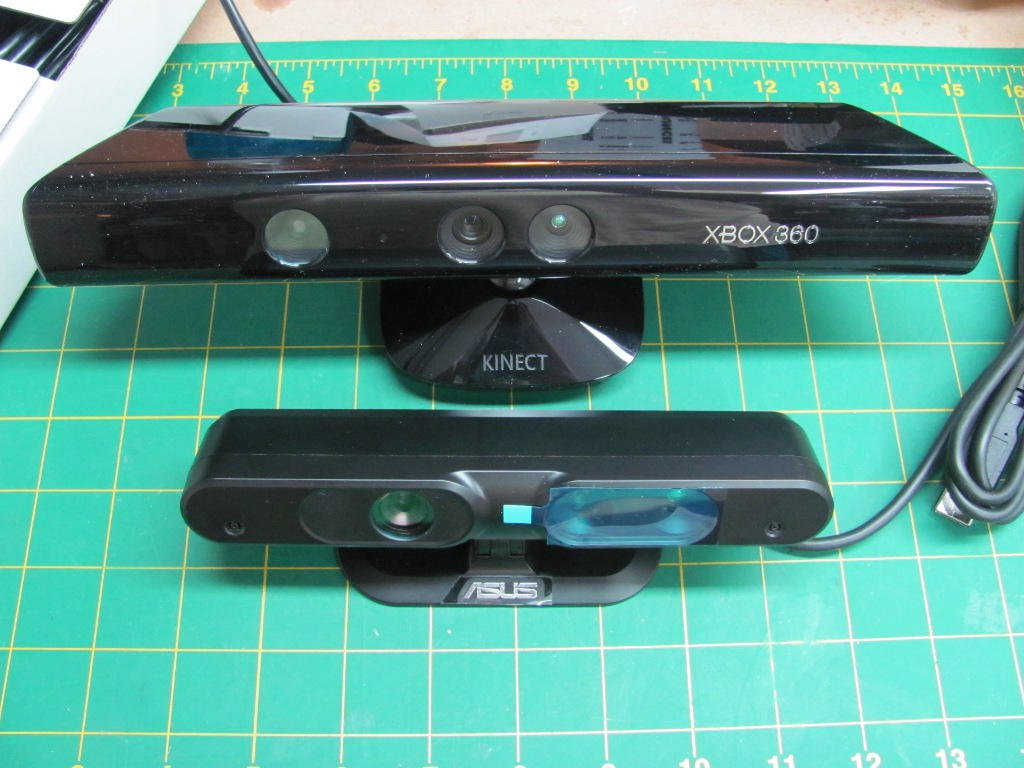
\includegraphics[width=3cm]{../images/kinect_vs_xtion.jpg} \hspace{1ex}
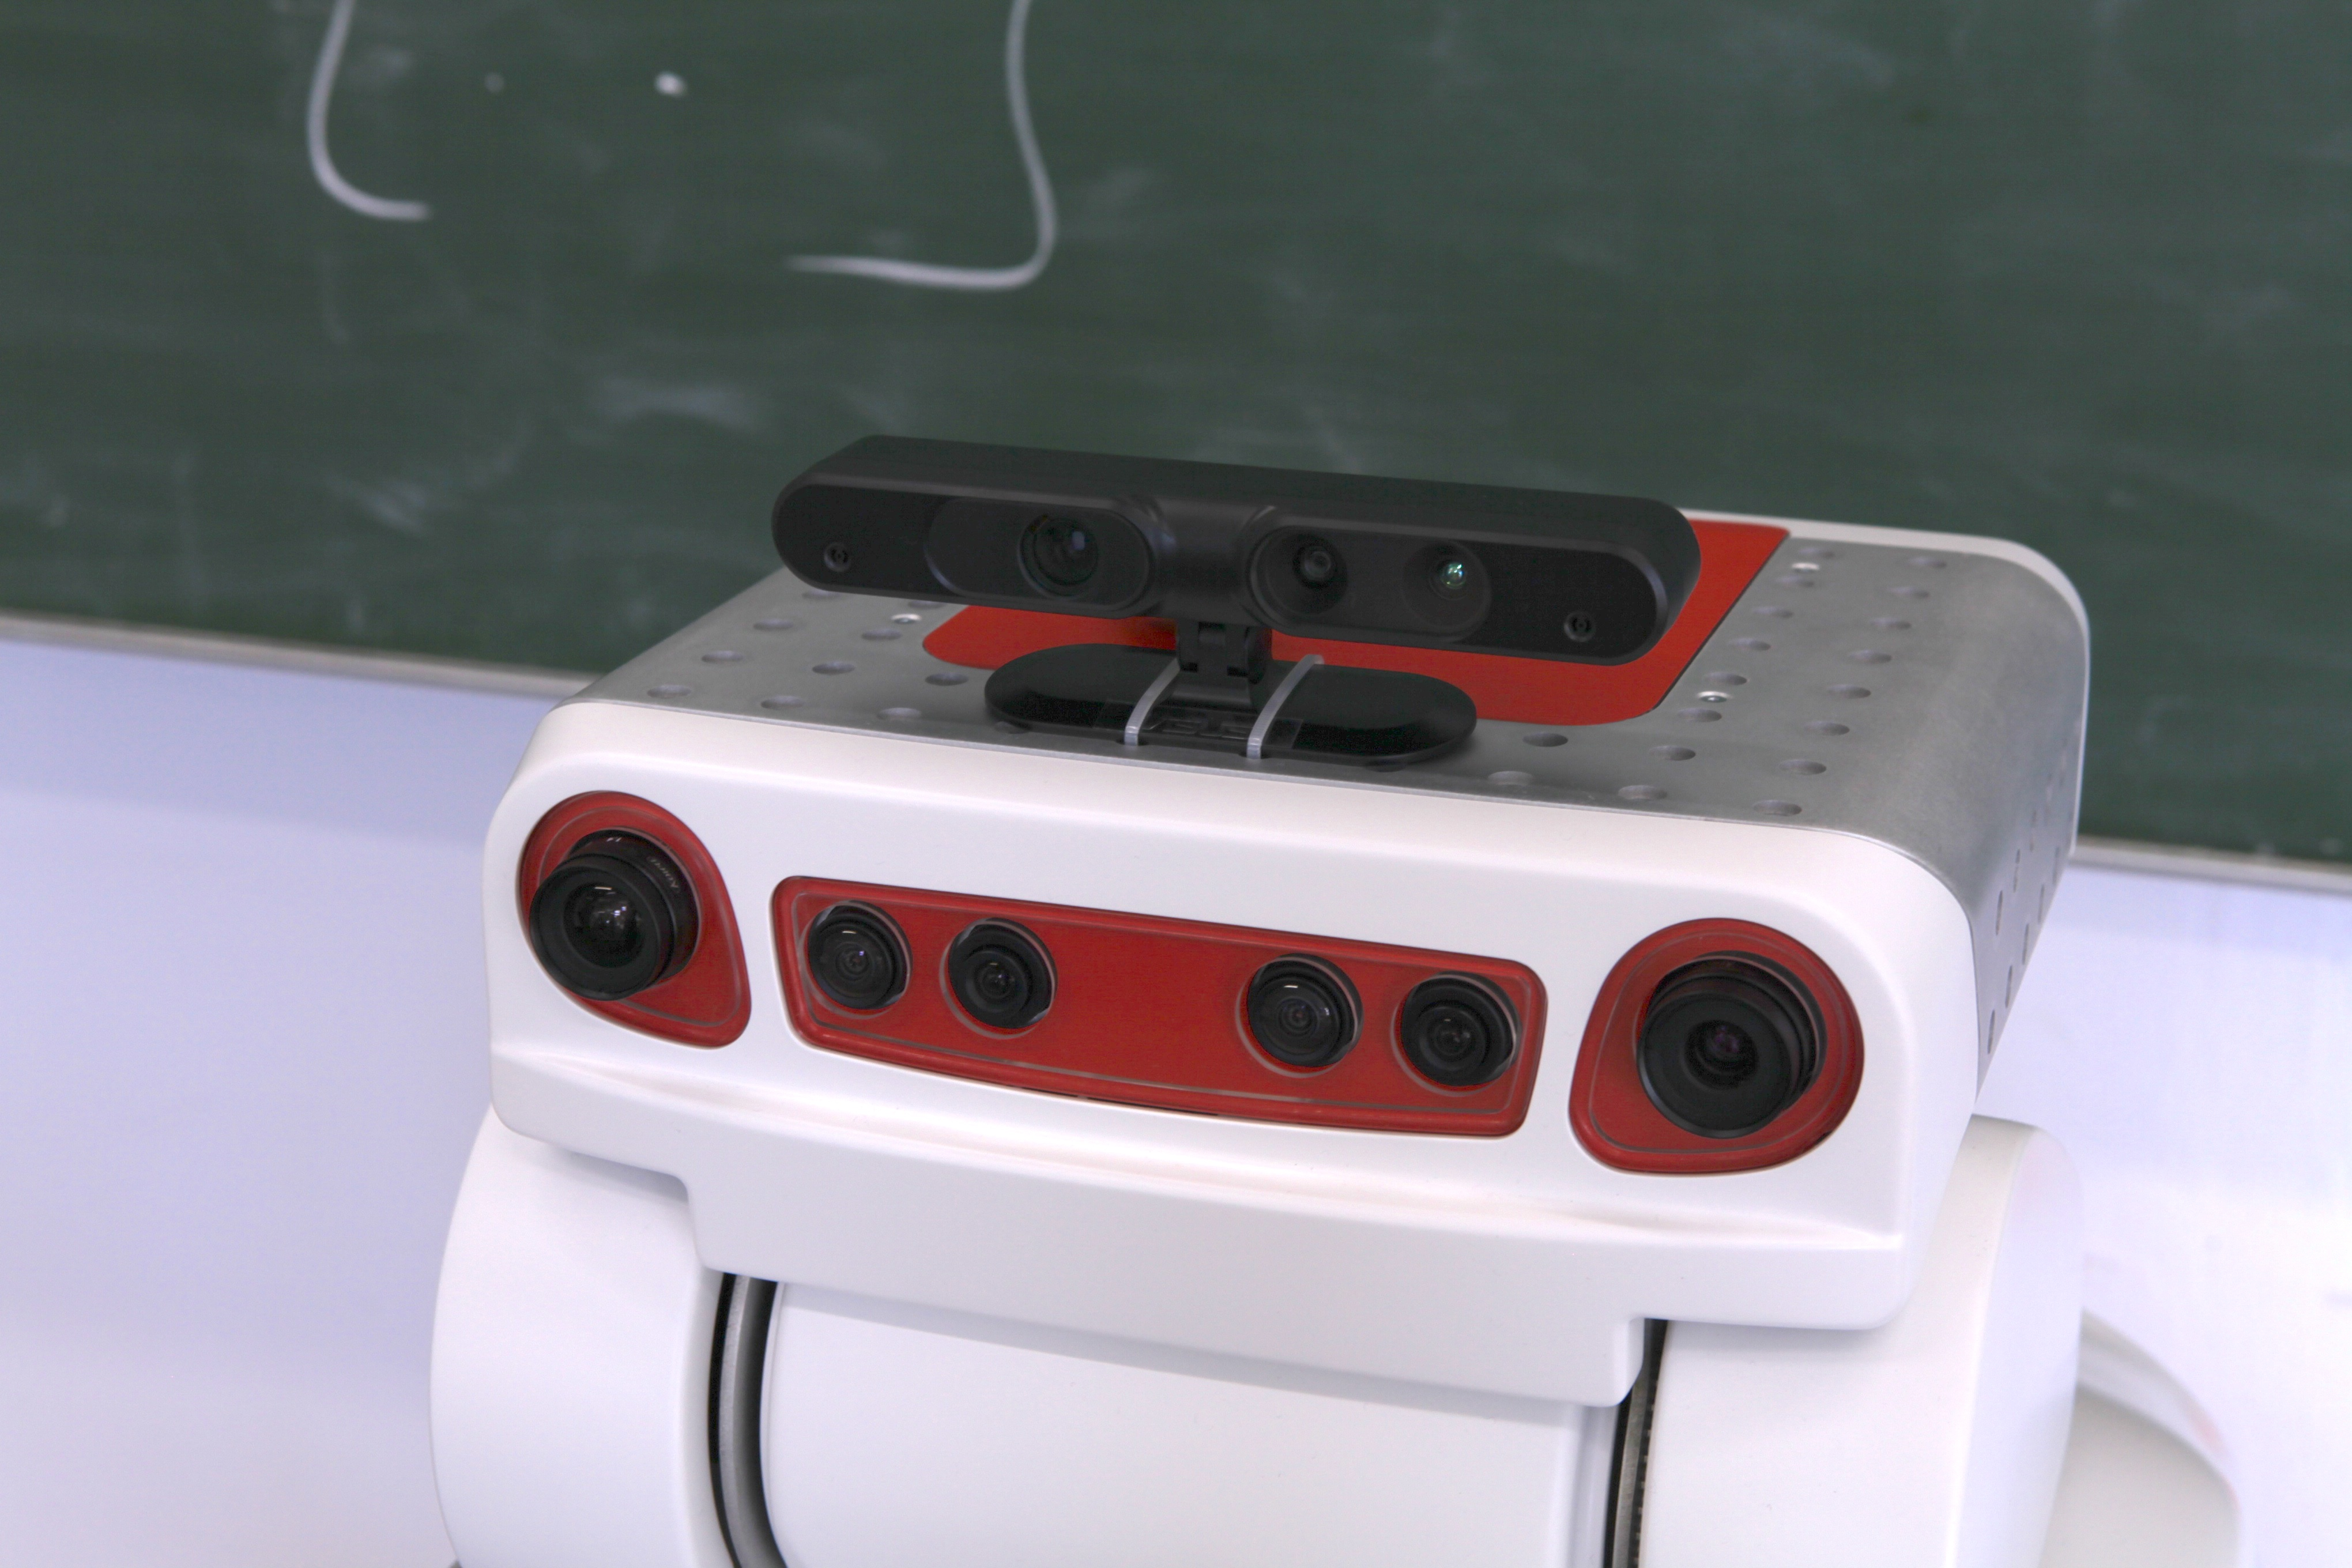
\includegraphics[width=3.38cm]{../images/IMG_1195.JPG} \hspace{1ex}
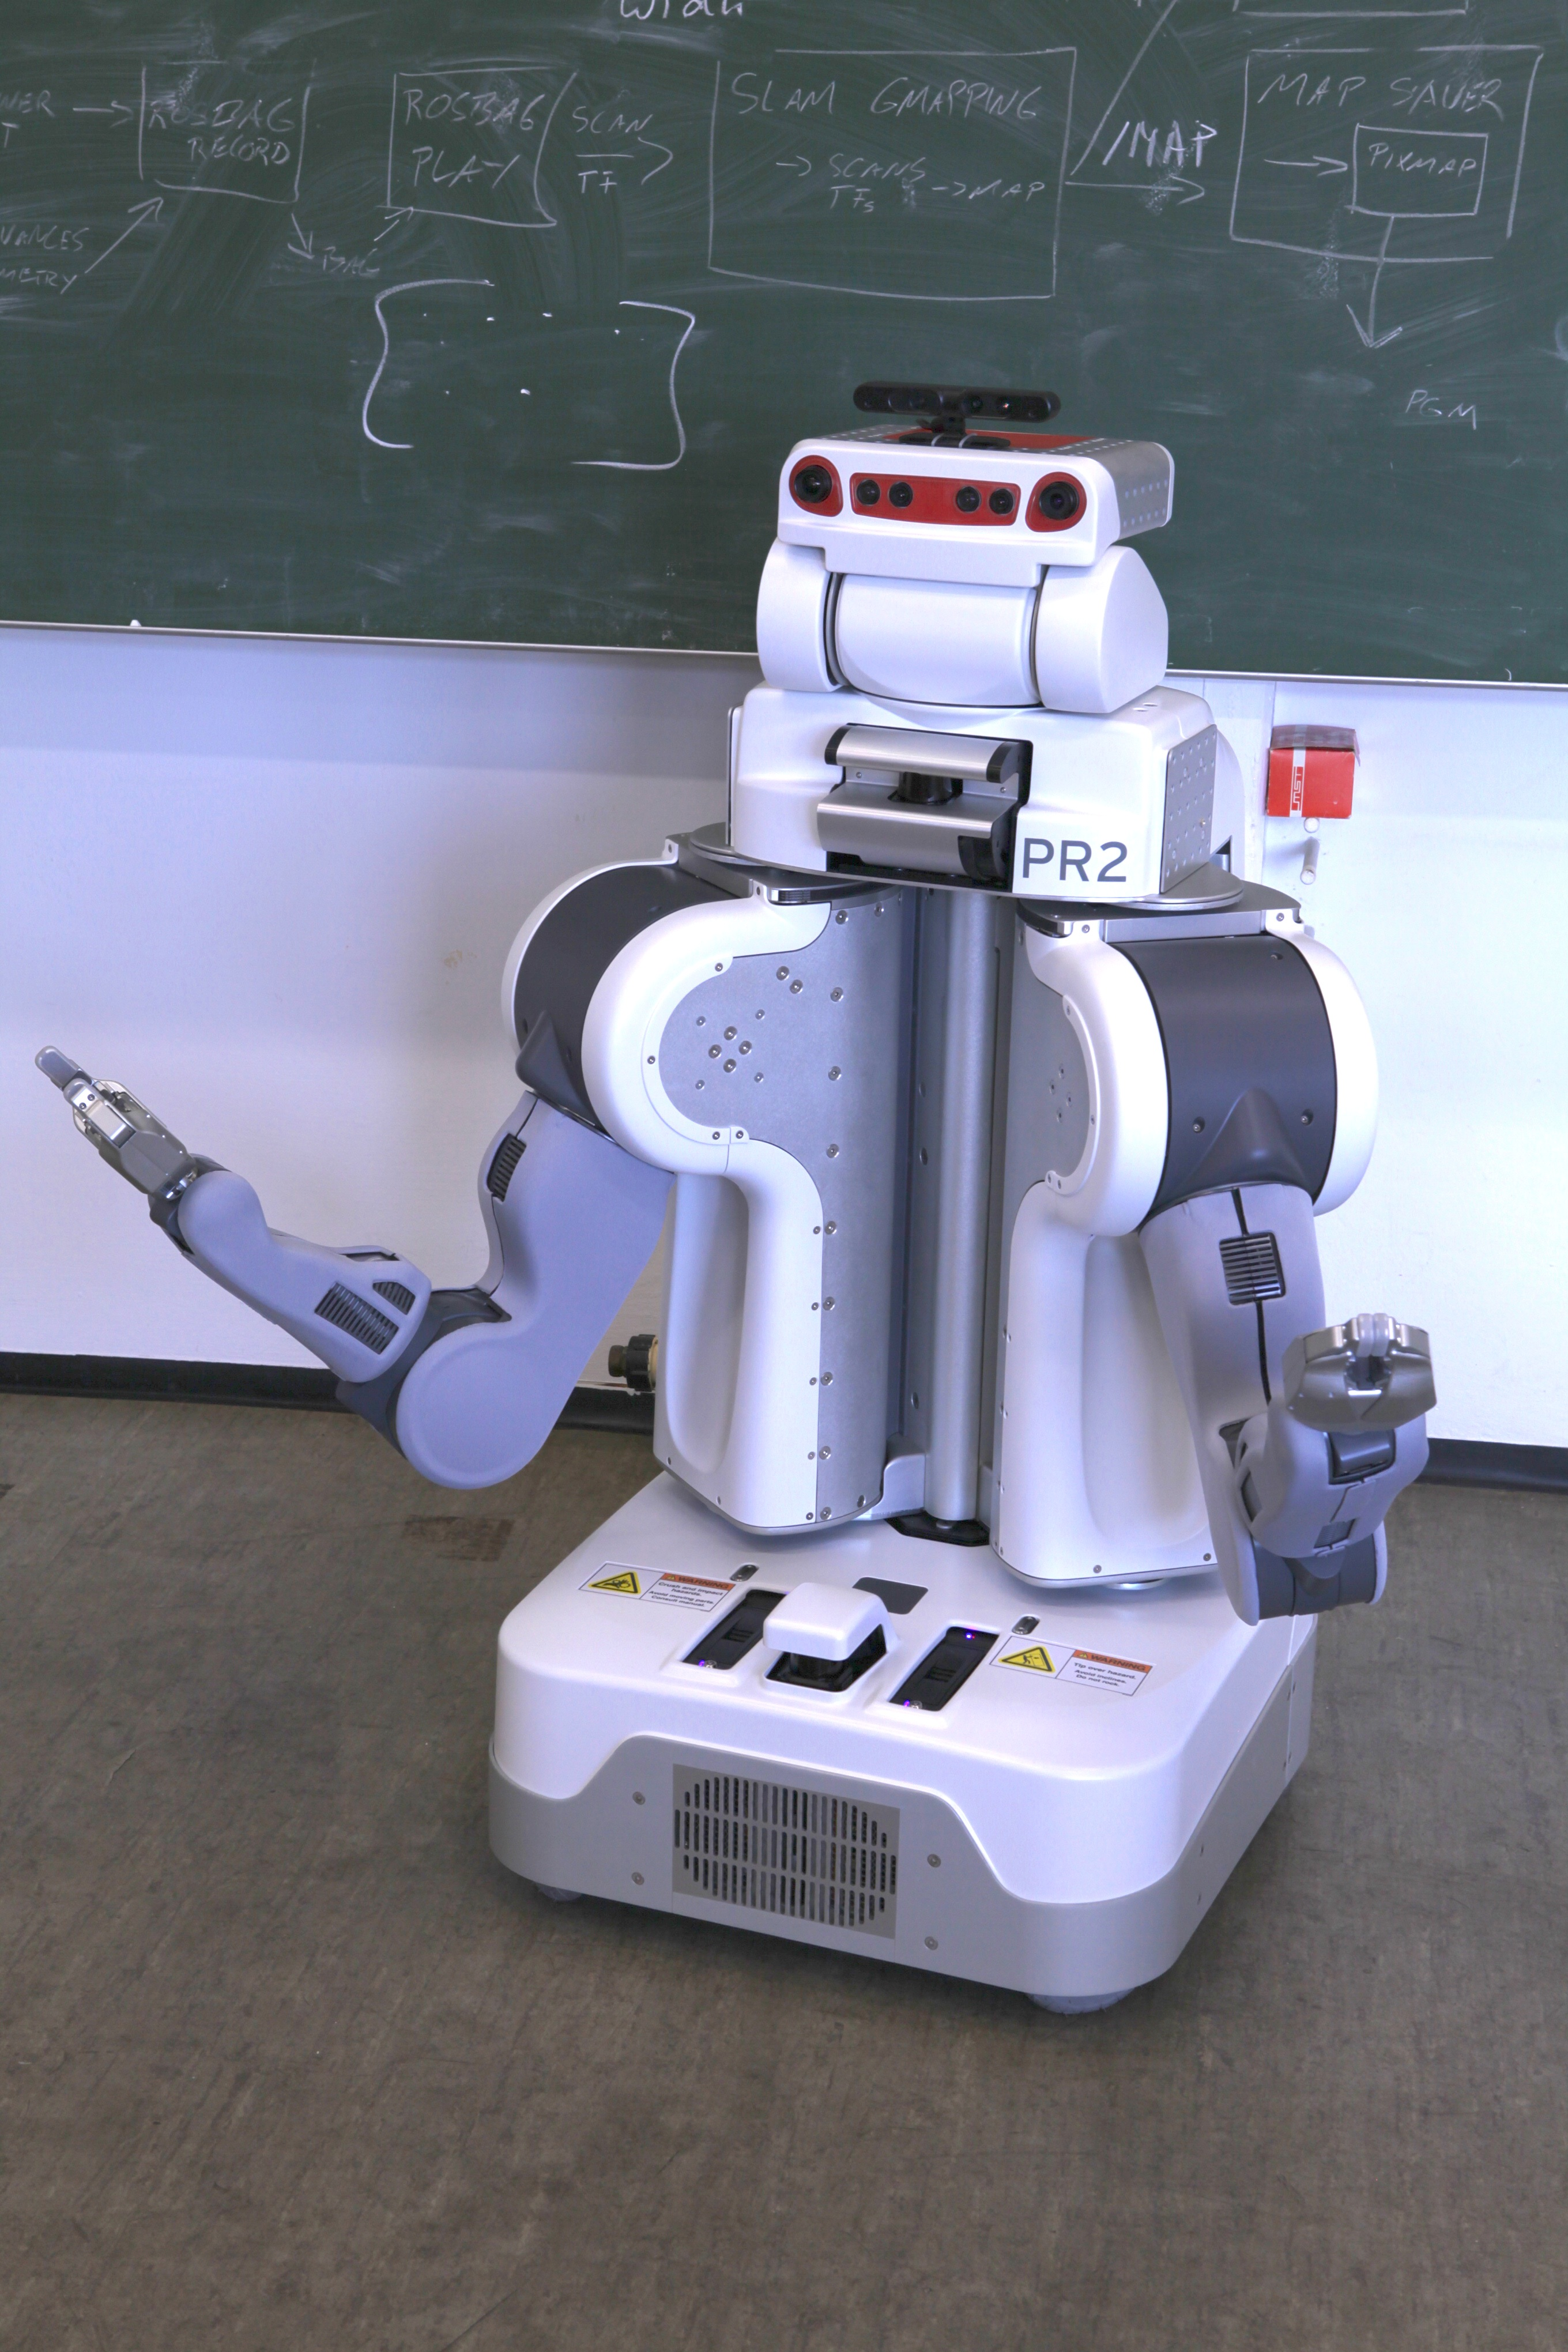
\includegraphics[width=1.5cm]{../images/IMG_1200.JPG}
\end{frame}

\subsection{ASUS Xtion Pro Live}
\begin{frame}
 \frametitle{ASUS Xtion Pro Live - technical details}
\begin{itemize}
  \item Resolution of (640 $\times$ 480) @ 30 Hz (color) and (320 $\times$ 240) @ 30 Hz (depth)
  \item Angular field of view of $58^0$ horizontally and $45^0$ vertically
  \item Range of approximately 0.8 - 3.5\,m (practical 0.7 - 3.5\,m)
  \item Voice microphone and array supporting single speaker voice recognition (16-bit audio @ 16 kHz)
  \item OpenNI drivers
\end{itemize}
\vspace{1ex}\hspace{39ex}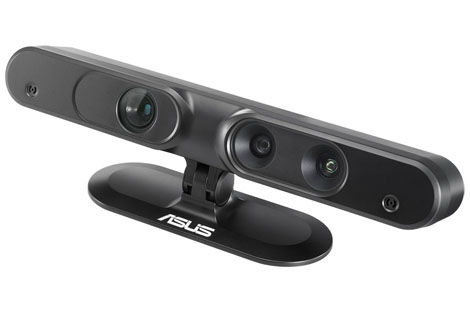
\includegraphics[width=4cm]{../images/asus_xtion.jpg}
\end{frame}

\begin{frame}
 \frametitle{ASUS Xtion Pro Live - first results}
%\vspace{1ex}\hspace{39ex}
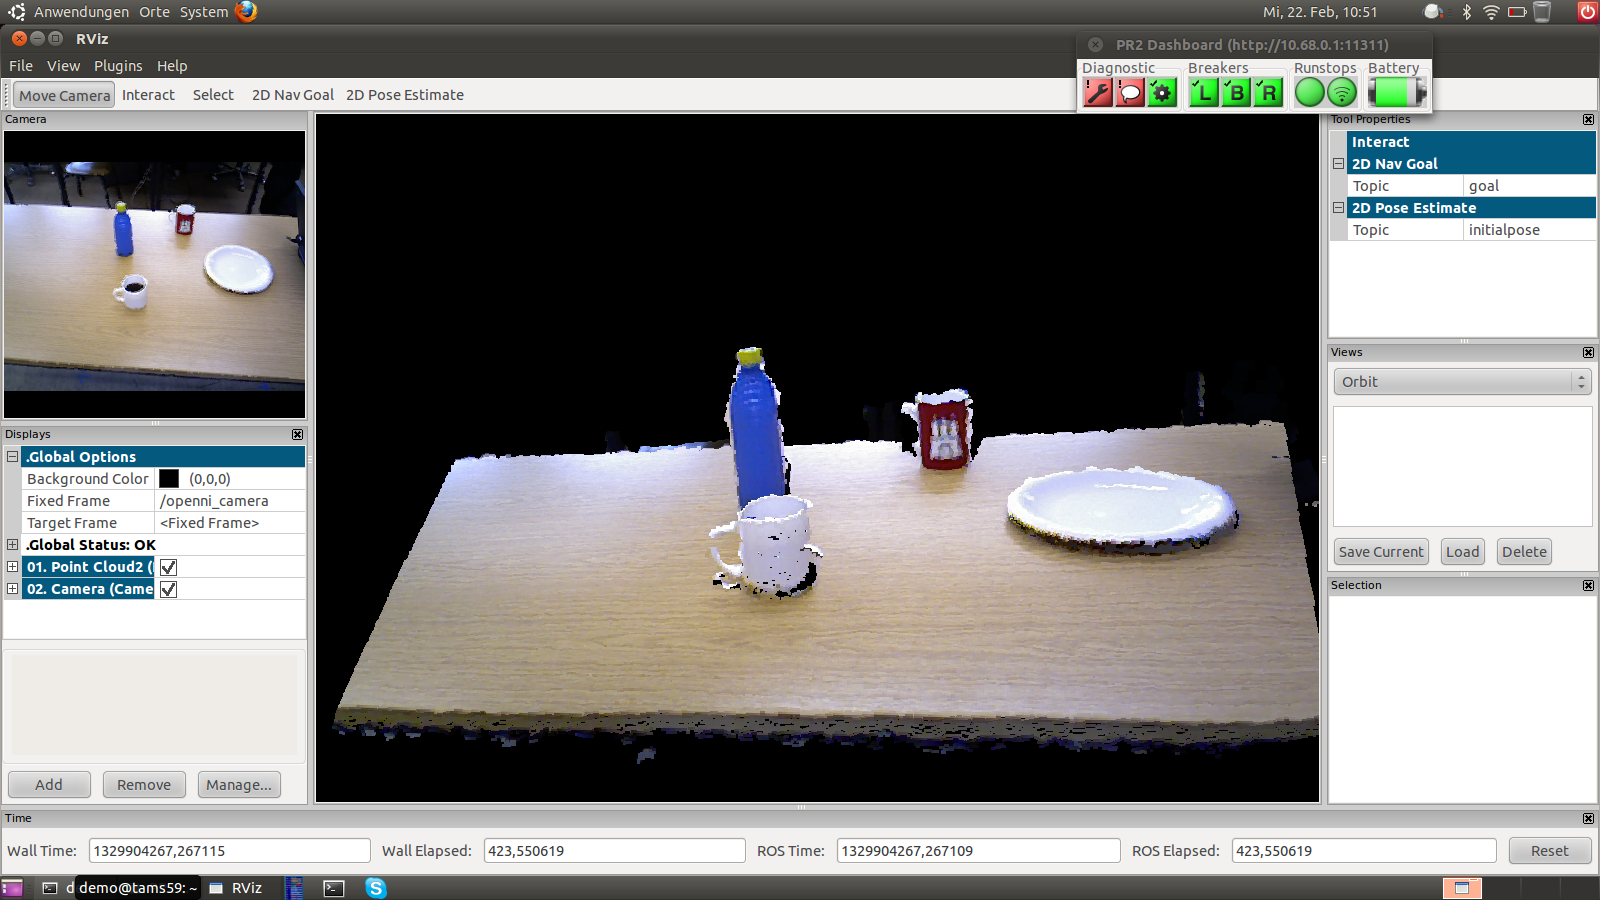
\includegraphics[width=11cm]{../images/asus2.png}
\end{frame}

\begin{frame}
 \frametitle{ASUS Xtion Pro Live - first results}
%\vspace{1ex}\hspace{39ex}
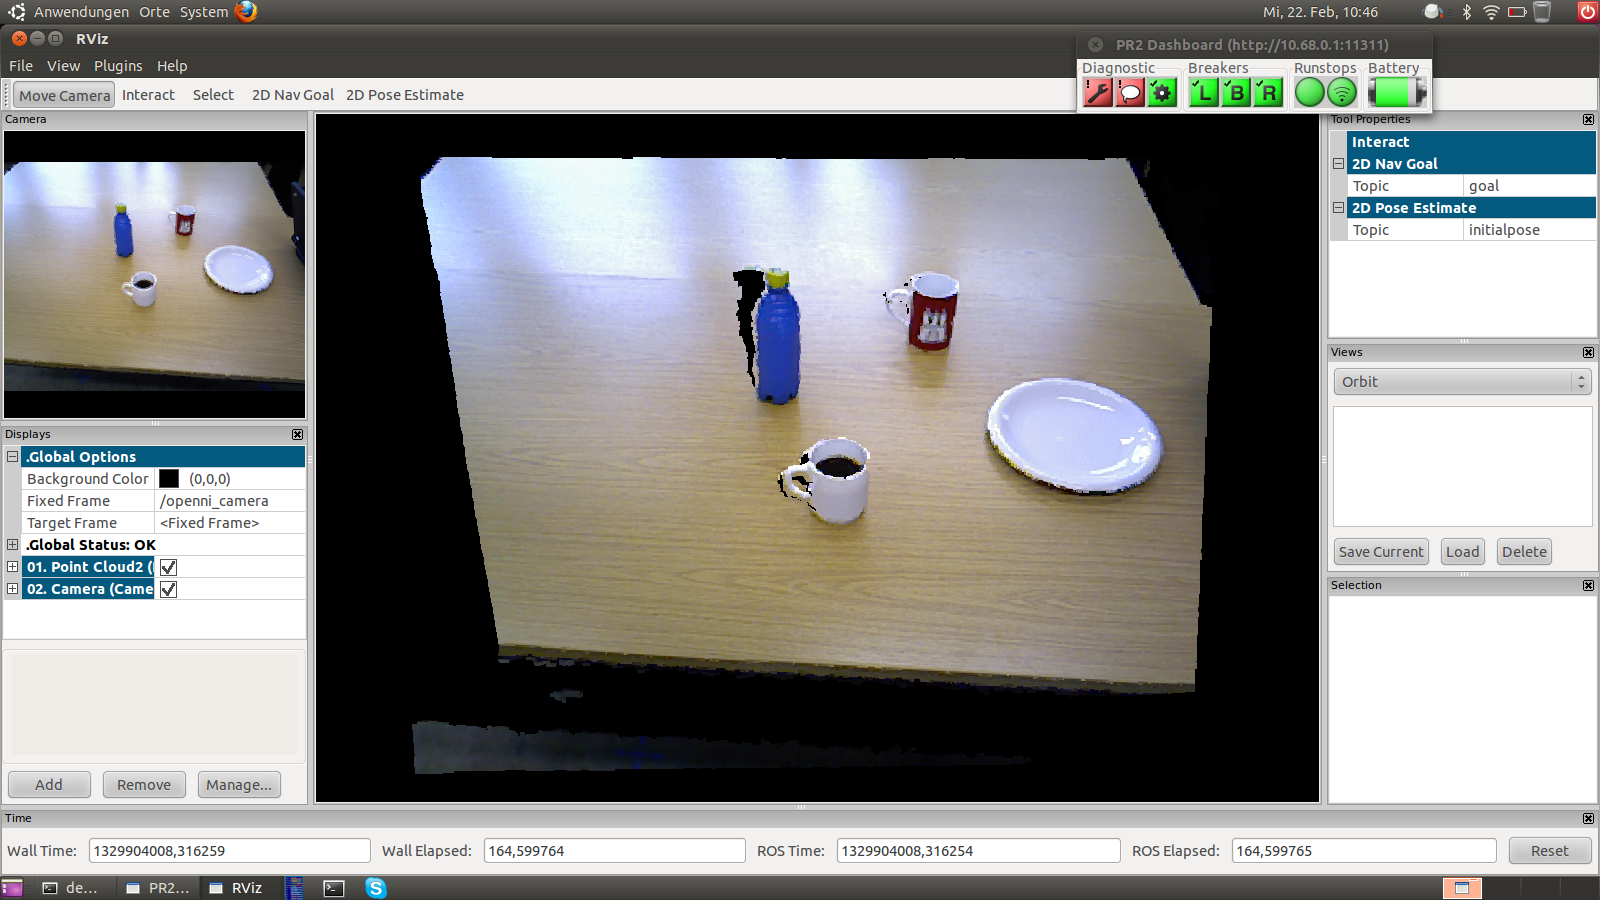
\includegraphics[width=11cm]{../images/asus1.png}
\end{frame}


\section{Available Sensor Information and Data Record}
\begin{frame}
 \frametitle{Available sensor information}
\begin{itemize}
 \item Fingertip pressure sensor ($4 \times 22$ values)
 \item Color information
 \item Wide stereo camera system (PointCloud)
 \item Narrow stereo camera system (LED textured light projector) (PointCloud)
 \item LRF in the Base (2D)
 \item Tilted LRF (PointCloud)
 \item Kinect or Asus Xtion Pro Live (Color and Depth) (PointCloud)
\end{itemize}

\end{frame}

\begin{frame}
 \frametitle{Data record and distribution}
 \begin{itemize}
  \item ROSBAG
  \item Set of tools for recording from ROS topics as well as playing back
  \item Possibilities to record of all data or partial
  \item Data rate from 0.53 MB/s (tf/Odom/2D LRF) to 50 MB/s (+ data from the Kinect/Asus) (all data)
  \item $2 \times$ hard disks with 1,5 TB respectively (in the base of the PR2)
  \item Planing to buy: 3 further hard disks and 2 hard disk mobile racks
 \end{itemize}

\end{frame}

%%%%%%%%%%%%%%%%%%%%%%%%%%%%%%%%%%%%%%%%%%%%%%%%%%%%%%%

\begin{frame}
\vspace{1cm}
\centering\textbf{Thanks for your attention!\\}
%\vspace{0.7cm}
%\centering\textbf{Any questions?\\}

%\vspace{4ex}\hspace{22ex}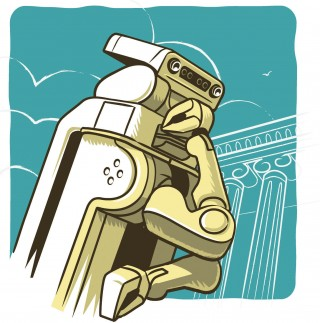
\includegraphics[width=3.5cm]{../images/thinker.jpg}
\vspace{4ex}\hspace{22ex}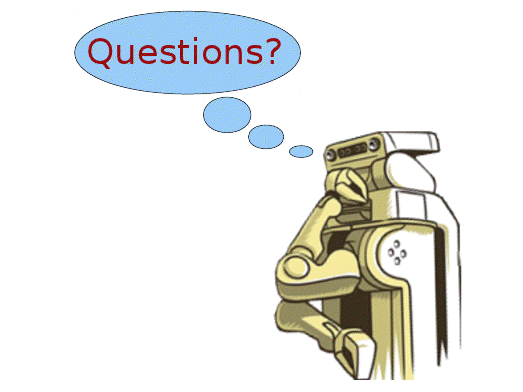
\includegraphics[width=5.5cm]{../images/pr2_questions.png}
\end{frame}
